%!Mode:: "TeX:UTF-8"
\section{测量工具汇总}

\subsection{网络流量测量}
\textbf{vnstat, sar, slurm, ifstat, system-monitor}等工具可查看网卡总流量。\textbf{iptraf,iftop}可查看连接的流量。
参考\ref{sec:netmeasure}。


\subsection{磁盘速率测量}
关于磁盘负载的生成器,主要有iometer和\textbf{iostat}。

本文使用Iometer工具评测存储设备性能。Iometer最初由英特尔公司开发,并得到了广泛应用。此后Iometer已经成为一个开源项目,在GPL协议下发布。本文中使用的Iometer工具包含两部分,分别为Linux下的负载发生器Dynamo和Windows PC下的控制端,该控制端也称为Iometer(以下用Iometer指代Windows下的控制端)。Dynamo在Linux运行时能够掌控本地的所有CPU核,并掌握已被加载的所有磁盘的情况。而Dynamo又为Iometer所控制,需要将每次I/O的运行状况随时报告给Iometer。Iometer与Dynamo通信,操纵Dynamo对目标磁盘发起读写访问,并控制I/O访问参数,如读/写比例,随机I/O与顺序I/O的选择,数据块的大小,核对磁盘分区的任务分配,测试时长,结果刷新频率等。Iometer的分析结果给出了磁盘I/O过程中的IOPS(每秒钟I/O次数)、数据速率、CPU利用率、延迟、错误率等参数的测量。

Iostat对磁盘IO操作进行监视,它仅分析系统整体状况,不对进程进行深入分析。

Iostat常常配合dd使用。以下命令在当前目录下生成一个50M的文件:
\begin{verbatim}
dd if=/dev/zero of=50M.file bs=1M count=50
\end{verbatim}
 


\subsection{内存消耗测量}
常用的内存测量工具为\textbf{free}。
此外,\textbf{top,ps}显示了各进程的内存使用信息。

\textbf{pmap}显示指定进程的内存映像信息:
\begin{verbatim}
pmap PID
\end{verbatim}

\begin{verbatim}
 free -m:内存使用率(-m 表示单位为MB而非KB)
\end{verbatim}
上述free命令中,m选项设置单位为MB。因为buffer和cache是否算作已用空间有争议,故分两种算法列出。
上述vmstat命令,M表示单位为MB,如果是m,则为1000*1000B。


 
\subsection{存储消耗测量}
常用的存储/文件系统测量工具为\textbf{df}和\textbf{du}。
 如果只想查看当前目录下所有子目录的大小,有
\begin{verbatim}
du -s
\end{verbatim}
或者
\begin{verbatim}
du -h --max-depth=1
\end{verbatim}



\subsection{综合测量工具vmstat}
vmstat(Virtual Memory Statistics)是最常见的Linux/Unix监控工具,可以展现给定时间间隔的服务器的状态值,包括服务器的CPU使用率,内存使用,虚拟内存交换情况,IO读写情况。
不足之处是无法对某个进程进行深入分析。

\begin{verbatim}
vmstat -d:磁盘信息
vmstat -s: slab信息
vmstat -p /dev/sda1 : 分区信息
\end{verbatim}

举例:
\begin{verbatim}
#vmstat 1 5
procs -----------memory---------- ---swap-- -----io---- -system-- ----cpu----
 r  b   swpd   free   buff  cache   si   so    bi    bo   in   cs us sy id wa
 0  0 235148 398516  40376 513916    0    3    28    17  291  107  5  2 93  1
 1  0 235148 398580  40376 513916    0    0     0     0  710 1337  8  1 92  0
 0  0 235148 403460  40384 508676    0    0     0   168 1065 4172 28  6 66  0
 0  0 235148 403320  40384 508648    0    0     0    24  759 1481  6  2 92  0
 0  0 235148 403416  40384 508648    0    0     0     0  691  952  7  2 92  0
\end{verbatim}
r表示运行和等待CPU时间片的个数,如长期超过CPU个数,说明压力过大。

\subsection{综合测量工具:sar}
sar(System Activity Report)是源于Solaris的系统监视命令,用于报告系统负载,包括CPU,内存,磁盘,网络\cite{wikipedia}。在Linux上通过sysstat软件包来提供。
与sysstat类似的工具还包括\textbf{atsar}和\textbf{dstat}。

Sysstat是一个工具集,包括\textbf{sar、pidstat、iostat、mpstat、sadf、sadc}。sadc(System Activity Data Collector)是sar的后端,为其收集数据。


\begin{verbatim}
pidstat  2   5  
// 每隔2秒,显示5次,所有活动进程的CPU 使用情况 
pidstat  - p  3132   2   5  
// 每隔2秒,显示5次,PID为1643的进程的CPU使用情况显示 
pidstat  - p  3132   2   5   - r
// 每隔2秒,显示5次,PID为1643的进程的内存使用情况显示
\end{verbatim}

\begin{verbatim}
sar 2 // 每隔2秒显示CPU使用的情况										
sar -r 2 //内存使用情况					 
sar -d 2 //磁盘使用情况					 
sar -n DEV  2 //网络使用情况
iostat 2 //磁盘使用情况
\end{verbatim}

\subsection{综合测量工具:top}
对于top命令,最重要的两个交互快捷键是h和q,分别打印帮助信息和退出top。利用好h命令就能够进行各种复杂操作。例如,F可以选择一个field列,以其为标准进行行排序,如n表示MEM。
k键可用杀进程。r键可用renice进程。


\begin{figure}[ht]
	\begin{center}
	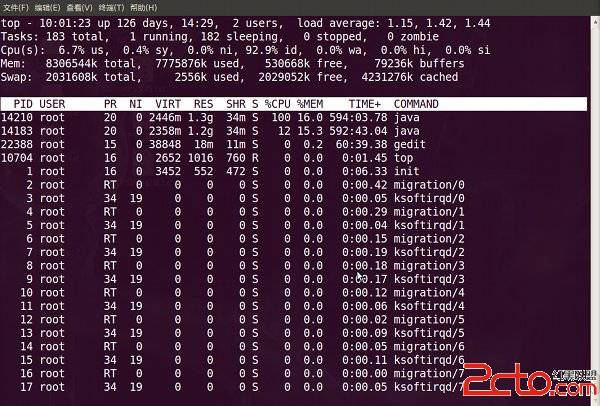
\includegraphics[keepaspectratio,width=0.6\paperwidth]{Pictures/topCmdUbuntu.jpg}
		\caption{top在ubuntu下的输出}
	\label{fig:topCmdUbuntu}
	\end{center}
\end{figure}

top的前五行显示整个系统的信息。

第一行:
 10:01:23 当前系统时间\\
 126 days, 14:29 系统已经运行了126天14小时29分钟(在这期间没有重启过)\\
 2 users 当前有2个用户登录系统\\
 load average: 1.15, 1.42, 1.44 load average后面的三个数分别是1分钟、5分钟、15分钟的负载情况。\\
load average数据是每隔5秒钟检查一次活跃的进程数,然后按特定算法计算出的数值。如果这个数除以逻辑CPU的数量,结果高于5的时候就表明系统在超负荷运转了。
  
第二行:
 Tasks 任务(进程),系统现在共有183个进程,其中处于运行中的有1个,182个在休眠(sleep),stoped状态的有0个,zombie状态(僵尸)的有0个。

第三行:cpu状态
\begin{itemize}
\item us 用户空间占用CPU的百分比。
\item sy 内核空间占用CPU的百分比。
\item ni 改变过优先级的进程占用CPU的百分比
\item id 空闲CPU百分比
\item wa IO等待占用CPU的百分比
\item hi 硬中断(Hardware IRQ)占用CPU的百分比
\item si 软中断(Software Interrupts)占用CPU的百分比
\end{itemize}

第四行:内存状态
\begin{itemize}
\item total 物理内存总量(8GB)
\item used 使用中的内存总量(7.7GB)
\item free 空闲内存总量(530M)
\item buffers 缓存的内存量 (79M)
\end{itemize}

第五行:swap交换分区
\begin{itemize}
\item  2031608k total 交换区总量(2GB)
\item  2556k used 使用的交换区总量(2.5M)
\item  2029052k free 空闲交换区总量(2GB)
\item  4231276k cached 缓冲的交换区总量(4GB)
\end{itemize}

第四行中使用中的内存总量(used)指的是现在系统内核控制的内存数,空闲内存总量(free)是内核还未纳入其管控范围的数量。纳入内核管理的内存不见得都在使用中,还包括过去使用过的现在可以被重复利用的内存,内核并不把这些可被重新使用的内存交还到free中去,因此在linux上free内存会越来越少,但不用为此担心。
如果出于习惯去计算可用内存数,这里有个近似的计算公式:第四行的free + 第四行的buffers + 第五行的cached,按这个公式此台服务器的可用内存:530668+79236+4231276 = 4.7GB。
  
对于内存监控,在top里我们要时刻监控第五行swap交换分区的used,如果这个数值在不断的变化,说明内核在不断进行内存和swap的数据交换,这是真正的内存不够用了。


top默认为每个进程显示以下信息:
PID(进程号)、 USER(运行用户)、PR(优先级)、NI(任务nice值)、VIRT(虚拟内存用量, VIRT=SWAP+RES) 、RES(物理内存用量)、SHR(共享内存用量)、S(进程状态)、\%CPU(CPU占用比)、\%MEM(物理内存占用比)、TIME+(累计CPU占用时间)、COMMAND 命令名/命令行。


一些交互式命令:
\begin{description}
    \item  [f] 进入另一个视图,在这里可以编排基本视图中的显示字段。
    \item  [k] 可以用PID来杀进程
    \item  [r] renice
    \item  [c] 显示完整的应用程序路径
    \item  [M] 按照内存占用率排序
    \item  [P] 按照CPU占用率排序
    \item  [T] 按照累积时间排序    
\end{description}



\subsection{Nagios}
Nagios是一款开源的免费网络监视工具,能有效监控Windows、Linux和Unix的主机状态,交换机路由器等网络设置,打印机等。在系统或服务状态异常时发出邮件或短信报警第一时间通知网站运维人员,在状态恢复后发出正常的邮件或短信通知。

Nagios是一个监视系统运行状态和网络信息的监视系统。Nagios能监视所指定的本地或远程主机以及服务,同时提供异常通知功能等。
Nagios可运行在Linux/Unix平台之上,同时提供一个可选的基于浏览器的WEB界面以方便系统管理人员查看网络状态,各种系统问题,以及日志等等。

\subsection{按名称分类}
\begin{description}
\item[*stat]: vmstat, iostat, ifstat, vnstat
\item[ip*]: iptop, iptraf
\item[*top]:iptop, ntop
\end{description}

dstat是iostat, vmstat, ifstat 三合一的工具,用来查看系统性能。sysstat是sar所在的工具包。
你可以这样使用:
\begin{verbatim}
alias dstat='dstat -cdlmnpsy'
\end{verbatim}













